\documentclass[usenames,dvipsnames, aspectratio=169, 9pt]{beamer}
\beamertemplatenavigationsymbolsempty
\setbeamertemplate{footline}[frame number]
\setbeamertemplate{section in toc}[sections numbered]
\usecolortheme[named=Plum]{structure}
\usefonttheme{serif}
\usepackage{amsmath, amsthm, amssymb, pgffor, multirow, booktabs, tabularx, multirow, graphicx, pgffor, arydshln}
\usepackage{booktabs}
\usepackage{kotex}
\usepackage{epstopdf}
\usepackage{grffile}


\author{Boyeon Kim}
\institute{Department of Mathematics, School of Mathematics and Computing \\ Mathematics \\ Yonsei University}
%\date{January 6, 2023}
\title{Reinforcement Learning Seminar}

\def\bs{\boldsymbol}
\usepackage{grffile}
\begin{document}

  \maketitle

\begin{frame}{SEIAR Optimal control}
    \begin{itemize}
        \item Goal1 : DQN
        \item Goal2 : PPO
    \end{itemize}
\end{frame}


\begin{frame}\frametitle{Mathematical models}
    \begin{itemize}
        \item The influenza model : SEIAR model 
        \item J.Kim et.al.,\textit{Constrained optimal control applied to vaccination for influenza},2016
    \end{itemize}
    \begin{align*}
        S'(t) &= -\beta S(t) \Lambda(t) - \psi \nu(t) S(t)\\
        E'(t) &= \beta S(t) \Lambda(t) - \kappa E(t)\\
        I'(t) &= p\kappa E(t) - \alpha I(t) - \tau I(t) \\
        A'(t) &= (1-p)\kappa E(t) - \eta A(t) \\
        R'(t) &= f \alpha I(t) + \tau I(t) + \eta A(t) + \psi \nu(t) S(t)
   \end{align*}
with $\Lambda(t) = \epsilon E(t) + (1 - q) I(t) + \delta A(t)$ 
    
    \centering
    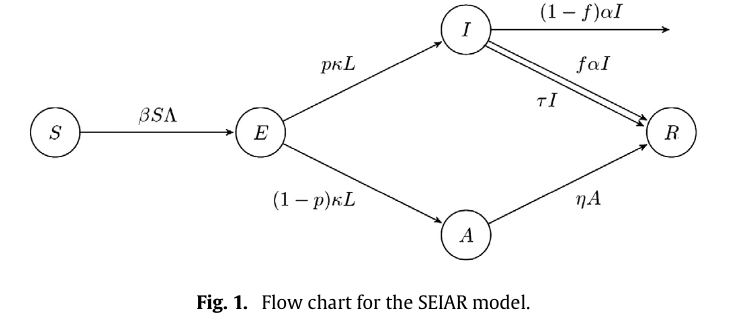
\includegraphics[width=8cm]{figures/model.png}
\end{frame}


\begin{frame}\frametitle{SEIAR model parameters}
\begin{table}[]
\begin{tabular}{lll}
\hline
Parameter & Description                                       & value        \\ \hline
$\epsilon$   & Infectivity reduction factor for the exposed      & 0            \\
$q$         & Contact reduction by isolation                    & 0.5          \\
$\delta$     & Infectivity reduction factor for the asymptomatic & 0.5          \\
$p$         & Fraction of developing symptoms                   & 0.667        \\
$\kappa$     & Transition rate for the exposed                   & 0.7143 / day \\
$f$         & Complement to fatality rate (1 - fatality rate)   & 0.999        \\
$\alpha$     & Recovery rate for the (symptomatic) infective     & 0.1667 /day  \\
$\eta$       & Recovery rate for the asymptomatic                & 0.1667 / day \\
$\tau$       & Antiviral treatment rate                          & 0 / day      \\
$\psi$       & Efficacy of vaccination                           & 70\%         \\ 
$\beta$    & Transmission rate                                 & 6.3346e-08           \\
$R_{0}$     & Basic Reproduction number                         & 1.9           \\\hline
\end{tabular}
\end{table}
\begin{itemize}
    \item $S0 = 5e07, \quad E0 = 0, \quad   I0 = 1,   \quad  A0 = 0,  \quad   R0 = 0$
\end{itemize}
\end{frame}


\begin{frame}\frametitle{Goal in paper}
\begin{itemize}
    \item The goal is to \textcolor{Plum}{\textbf{minimize the number of people who becom infected}} at a \textbf{minimal efforts of vaccination}.
    \item The objective functional is given by
\end{itemize}
\begin{align*}
J(\nu) = \int_0^T P I(t) + Q \nu^2(t) dt\\
\end{align*}
with
$0 \leq \nu(t) \leq 1$ , $\nu(t) S(t) \leq \nu_{max}$, $\int_0^T \nu(t) S(t) \leq \nu_{total}$
\end{frame}


% \begin{frame}\frametitle{SLIAR optimal control}
% \begin{align*}
% \min_{u\in\mathcal{U}_{ad}} \int_0^T PI(t) + Q\nu^2(t) + R\tau^2(t) + W\sigma^2(t) dt
% \end{align*}

%     subject to 
%     \begin{align*}
%     \begin{cases}
%         S' &= -\beta (1-\sigma) S\Lambda - \nu S\\
%         L' &= \beta (1-\sigma) S\Lambda - \kappa L\\
%         I' &= p\kappa L - \alpha I - \tau I \\
%         A' &= (1-p)\kappa L - \eta A \\
%    \end{cases} \qquad with \quad \Lambda = \epsilon L + (1 - q) I + \delta A
%    \end{align*}
% \end{frame}


% \begin{frame}\frametitle{SLIAR optimal control : multicontrol(nu+tau+sigma)}
% \begin{itemize}
% \item $ \min_{u\in\mathcal{U}_{ad}} \int_0^T PI(t) + Q\nu^2(t) + R\tau^2(t) + W\sigma^2(t) dt$
% \item Method : DQN (learning rate : 5e-4)
% \item $\nu_{max} = 0.01$, $\tau_{max} = 0.05$,  $\sigma_{max} = 0.01$
% \end{itemize}
% \centering
%     \includegraphics[width=6cm]{figure/2023-04-14/03-34-57/0/figures/all_best.png}
%     \includegraphics[width=6cm]{figure/2023-04-14/03-34-57/0/SLIAR_score.png}
% \end{frame}

% \begin{frame}{Last session discussion}
%     \begin{itemize}
%         \item Issue : Good learning? 
%         \item Check 1 : Change the weight
%     \end{itemize}
% \end{frame}

% \begin{frame}\frametitle{SLIAR optimal control : multicontrol(nu+tau+sigma)}
% \begin{itemize}
% \item $ \min_{u\in\mathcal{U}_{ad}} \int_0^T PI(t) + Q\nu^2(t) + R\tau^2(t) + W\sigma^2(t) dt$
% \item Method : DQN (learning rate : 5e-4)
% \item $\nu_{max} = 0.01$, $\tau_{max} = 0.05$,  $\sigma_{max} = 0.01$
% \end{itemize}
% \centering
%     \includegraphics[width=6cm]{figure/2023-04-14/03-34-57/1/figures/all_83000.png}
%     \includegraphics[width=6cm]{figure/2023-04-14/03-34-57/1/SLIAR_score.png}
% \end{frame}

% \begin{frame}\frametitle{SLIAR optimal control : multicontrol(nu+tau+sigma)}
% \begin{itemize}
% \item $ \min_{u\in\mathcal{U}_{ad}} \int_0^T PI(t) + Q\nu^2(t) + R\tau^2(t) + W\sigma^2(t) dt$
% \item Method : DQN (learning rate : 5e-4)
% \item $\nu_{max} = 0.01$, $\tau_{max} = 0.05$,  $\sigma_{max} = 0.01$
% \end{itemize}
% \centering
%     \includegraphics[width=6cm]{figure/2023-04-14/03-34-57/3/figures/all_6000.png}
%     \includegraphics[width=6cm]{figure/2023-04-14/03-34-57/3/SLIAR_score.png}
% \end{frame}

% \begin{frame}{Next}
%     \begin{itemize}
%         \item Issue : Good learning? 
%         \item Check 2 : Change the replay buffer
%     \end{itemize}
% \end{frame}


\end{document}